\documentclass[crop,tikz]{standalone}
\usetikzlibrary{backgrounds}
\colorlet{blue}{cyan}
\tikzset{
  inverted/.style = {
    color=white,
    background rectangle/.style={fill},
    show background rectangle
  }
}
\usepackage{pgfplots}

\usetikzlibrary{arrows.meta}

% Vector field of a homogeneously electrically charged and rotating
% sphere of Radius R. In spherical coordinates, the magnetic field is
%
% \vec{B}(r,\theta,\varphi)
%   = \mu_0 m/(4\pi r^3)[3\vec{e}_r(\vec{e}_z\cdot\vec{e}_r) - \vec{e}_z]
%   = \mu_0 m/(4\pi r^3)[2\cos(\theta)\vec{e}_r + \sin(\theta)\vec{e}_\theta],
%
% where m = q\omega R^2/3 is the magnetic moment, q is the total
% charge of the sphere, \omega is the angular frequency of the
% rotation and \theta\in[0;\pi] and \varphi\in[0;2\pi). In cartesian
% coordinates one has
%
% \vec{B}(x,y,z)
%   = \mu_0 m/(4\pi r^5)[3xz\vec{e}_x + 3yz\vec{e}_y + (2z^2 - x^2 - y^2)\vec{e}_z].

\pgfplotsset{
  compat=1.18,
  inverted/.style = {
    every axis legend/.append style={
      draw=white,
      fill=black,
      text=white
    }
  },
}

\usetikzlibrary{decorations.markings,arrows.meta}

\tikzset{
  fieldline/.style={
    red,
    thin,
    postaction={decorate},
    decoration={
      markings,
      mark=at position 0.5 with {\arrow{Latex[length=1mm]}}
    }
  },
}

\begin{document}
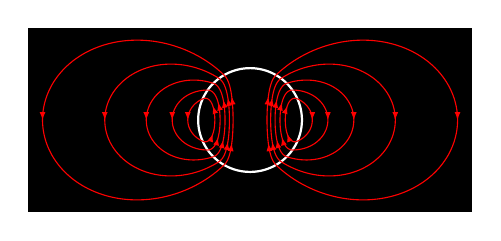
\begin{tikzpicture}[inverted,inverted]
  \begin{axis}[inverted,
    hide axis,
    axis equal image,
    xlabel={$x$},
    ylabel={$z$},
    xmin=-5.2, xmax=5.2,
    ymin=-3.2, ymax=3.2,
    samples=150,
    clip=false,
    ]
    % radius of sphere
    \pgfmathsetmacro{\R}{1}
    % sphere
    \addplot[white, thick, domain=0:360] ({\R*cos(x)}, {\R*sin(x)});
    % parameter
    \pgfplotsinvokeforeach{1.2,1.5,2,2.8,4}{
        % -------------------------
        % outside sphere
        % r = c sin^2(theta)
        % -------------------------
        \pgfmathsetmacro{\c}{#1}
        \pgfmathsetmacro{\cmin}{asin(sqrt(\R/\c))}
        \pgfmathsetmacro{\cmax}{180-\cmin}
        % right fieldline
        \addplot[
          fieldline,
          domain={\cmin}:{\cmax},
        ] ({\c*sin(x)^3}, {\c*sin(x)^2*cos(x)});
        % left fieldline
        \addplot[
          fieldline,
          domain={\cmin}:{\cmax},
        ] ({-\c*sin(x)^3}, {\c*sin(x)^2*cos(x)});
        % -------------------------
        % inside sphere
        % u(5-3u) sin^2(theta) = K
        % where u = r^2/R^2 and K = 2R/c
        % -------------------------
        \pgfmathsetmacro{\K}{2*\R/\c}
        % radius at equator
        % u_e is the smallest solution of u(5-3u)=K
        \pgfmathsetmacro{\ue}{(5 - sqrt(25 - 12*\K))/6}
        % upper right inner fieldline from equator to north
        \addplot[
          fieldline,
          domain={\ue}:1,
        ] ({\R*sqrt(\K/(5-3*x))}, {\R*sqrt(x)*sqrt(max(0,1-\K/(x*(5-3*x))))});
        % lower right inner fieldline from south to equator
        \addplot[
          fieldline,
          domain=1:{\ue},
        ] ({\R*sqrt(\K/(5-3*x))}, {-\R*sqrt(x)*sqrt(max(0,1-\K/(x*(5-3*x))))});
        % upper left inner fieldline
        \addplot[
          fieldline,
          domain={\ue}:1,
        ] ({-\R*sqrt(\K/(5-3*x))}, {\R*sqrt(x)*sqrt(max(0,1-\K/(x*(5-3*x))))});
        % lower left inner fieldline
        \addplot[
          fieldline,
          domain=1:{\ue},
        ] ({-\R*sqrt(\K/(5-3*x))}, {-\R*sqrt(x)*sqrt(max(0,1-\K/(x*(5-3*x))))});
    }
\end{axis}
\end{tikzpicture}
\end{document}
